\chapter{Logica}

\section{Relazioni}

\begin{define}[Prodotto cartesiano]
  Siano $A$ e $B$ due insiemi. Si definisce \textbf{prodotto cartesiano} di $A$ e $B$ l'insieme di coppie ordinate:

  $$
    A \times B = \{(a, b)~\colon~a \in A \wedge b \in B\}
  $$
\end{define}

\begin{define}[Relazione]
  Dati due insiemi $A$ e $B$ si definisce \textbf{relazione} $\mathfrak{R}$ tra $A$ e $B$ un 
  sottoinsieme del prodotto cartesiano $A \times B$. Diciamo che $\mathfrak{R}$ \textbf{associa} un elemento 
  $a \in A$ a $b \in B$ se $(a, b) \in \mathfrak{R}$.
\end{define}

\begin{notation}
  $A \mathfrak{R}B$
\end{notation}

\begin{define}[Funzione]
  Dati due insiemi $A$ e $B$, una funzione $f$ è una relazione che a 
  un elemento di $A$ associa al più un elemento di $B$.
\end{define}

\begin{notation}
  $f : A \to B$
\end{notation}


\section{Insiemi numerici}

\begin{define}[Estremo superiore]
  Sia $A \subset \mathbb{R}$, si definisce estremo superiore di $A$:

  \begin{itemize}
    \item $\sup_A := l \in \mathbb{R} \iff l \geqslant a~\forall a \in A~\wedge~\forall \varepsilon > 0~\exists a \in A~\colon~a \geqslant l - \varepsilon$
    \item $\sup_A := +\infty \iff \forall M > 0~\exists a \in A~\colon~a > M$
  \end{itemize}
\end{define}

\begin{define}[Massimo]
  Sia $A \subset \mathbb{R}$, si definisce massimo di $A$:

  $$
    \max{A} = M \in \mathbb{A}~\colon~M \geqslant a~\forall a \in \mathbb{A}
  $$
\end{define}

\begin{obs}
  Se $\sup_A \in \mathbb{A}, \sup_A = \max{A}$.
\end{obs}

\begin{axiom}[Assioma di completezza]
  Sia $A \subset \mathbb{R}$, $A \neq \emptyset$, con $A$ superiormente limitato. $A$ ammette estremo superiore in $\mathbb{R}$.
\end{axiom}


\section{Strutture algebriche}

\begin{define}[Campo]

\end{define}

\begin{define}[Relazione d'equivalenza]

\end{define}

\begin{define}[Relazione d'ordine]

\end{define}

\begin{define}[Campo ordinato]

\end{define}

\begin{define}[Campo ordinato completo]

\end{define}

\section{Sommatorie e produttorie}

\begin{notation}
  Sia $n \in \mathbb{N}_0$:

  \begin{itemize}
    \item $\displaystyle \sum_{n=1}^m a_n = a_1 + a_2 + \dots + a_m$
    \item $\displaystyle \prod_{n=1}^m b_n = b_1 \cdot b_2 \cdot \dots \cdot b_m$
  \end{itemize}
\end{notation}

\begin{prop}\leavevmode
  \begin{enumerate}[(I)]
    \item $\displaystyle \sum_{j=1}^n ca_j = c\sum_{j=1}^n a_n~\forall c \in \mathbb{C}$
    \item $\displaystyle \prod_{j=1}^n cb_j = c^n\prod_{j=1}^n b_j~\forall c \in \mathbb{C}$
    \item $\displaystyle \sum_{j=1}^n a_j + \sum_{j=1}^n b_j = \sum_{j=1}^n (a_j + b_j)$
    \item $\displaystyle \left(\prod_{j=1}^n a_j\right) \cdot \left(\prod_{j=1}^n b_j\right) = \prod_{j=1}^n (a_j \cdot b_j)$
    
    \item $\displaystyle \sum_{j=1}^{n+1} a_j = a_{n+1} + \sum_{j=1}^n a_j$
    \item $\displaystyle \prod_{j=1}^{n+1} b_j = b_{n+1} \cdot \prod_{j=1}^n b_j$
    
    \item $\displaystyle \sum_{j=1}^n a_j = \sum_{j=1+m}^{n+m} a_{j-m}~\forall m \in \mathbb{N}$
    \item $\displaystyle \prod_{j=1}^n b_j = \prod_{j=1+m}^{n+m} b_{j-m}~\forall m \in \mathbb{N}$

    \item $\displaystyle \sum_{j=0}^n a_j = \sum_{j=0}^{n} a_{n-j}$
    \item $\displaystyle \prod_{j=0}^n b_j = \prod_{j=0}^{n} b_{n-j}$
  \end{enumerate}
\end{prop}


\section{Principio di induzione}

\begin{principle}[Principio di induzione]
  Sia $p(n)$ una proposizione, con $n \in \mathbb{N}$. Se:

  \begin{itemize}
    \item $p(n_0)$ è verificata, con $n_0 \in \mathbb{N}$
    \item se $p(n)$ è vera, allora $p(n+1)$ è vera  
  \end{itemize}

  allora $p(n)$ è vera $\forall n \geqslant n_0$.
\end{principle}


\subsection{Disuguaglianza di Bernoulli}

\begin{thm}[Disuguaglianza di Bernoulli]
  Sia $x \in \mathbb{R}$ con $x > -1$, allora:

  $$
    (1 + x)^n \geqslant 1 + nx~\forall n \geqslant 1
  $$
\end{thm}

\begin{proof}
  Si proceda per induzione:

  \begin{itemize}
    \item $n = 1$: $(1 + x) \geqslant 1 + x$
    \item si supponga ora vera $P(n)$:
          \begin{align*}
            (1 + x)^{n+1} = (1+x)(1+x)^n  &\geqslant (1+x)(1+nx) = 1 + x(n+1) + \geqto{nx^2}{0} \\
                                          &\geqslant 1 + x(n+1)
          \end{align*}
  \end{itemize}
\end{proof}


\subsection{Fattoriale}

\begin{define}
  Sia $n \in \mathbb{N}$, si definisce \textbf{fattoriale} di n:

  $$
    n! := 
    \begin{cases}
      1~\text{se}~n = 0 \\
      n(n-1)~\text{se}~n > 0
    \end{cases}
  $$
\end{define}

\begin{define}
  Siano $k, m \in \mathbb{N}$ t.che $0 \leqslant k \leqslant n$, si definisce \textbf{coefficiente binomiale}:

  $$
    \binom{n}{k} := \dfrac{n!}{k!(n-k)!}
  $$
\end{define}

\begin{prop}
  Siano $0 \leqslant k \leqslant m$:

  \begin{enumerate}[(I)]
    \item $\displaystyle \binom{n}{k} = \binom{n}{n-k}$ (simmetria)
    \item $\displaystyle \binom{n}{k} + \binom{n}{k+1} = \binom{n+1}{k+1}$ (formula di Stiffer)
  \end{enumerate}
\end{prop}

\begin{proof}

\end{proof}


\begin{thm}[Formula del binomio di Newton]
  Sia $n \in \mathbb{N}_0$ e $a, b \in \mathbb{C}$, allora:

  $$
    (a + b)^n = \sum_{k=0}^n \binom{n}{k} a^k b^{n-k}
  $$
\end{thm}

\begin{proof}
  Si proceda per induzione:

  \begin{itemize}
    \item $(a + b)^0 = 1\cdot a^0 b^0 = 1$
    \item Si supponga ora vera $P(n)$:
          \begin{align*}
            (a + b)^{n+1} = (a+b)(a+b)^n  &= (a + b)\sum_{k=0}^n \binom{n}{k} a^k b^{n-k} \\
                                          &= \sum_{k=0}^n \binom{n}{k} a^{k+1} b^{n-k} + \sum_{k=0}^n \binom{n}{k} a^k b^{n+1-k} \\
                                          &= \sum_{k=1}^{n+1} \binom{n}{k-1} a^{k} b^{n+1-k} + \sum_{k=0}^n \binom{n}{k} a^k b^{n+1-k} \\
                                          &= \binom{n+1}{n} a^{n+1}b^{0} + \sum_{k=1}^{n} \binom{n}{k-1} a^{k} b^{n+1-k} + \sum_{k=1}^n \binom{n}{k} a^k b^{n+1-k} + \binom{n}{0}a^0b^{n+1} = \\
                                          &= \binom{n+1}{n+1} a^{n+1}b^{0} + \sum_{k=1}^{n}\left[\binom{n}{k-1} + \binom{n}{k}\right]a^{k} b^{n+1-k} + \binom{n}{0}a^0b^{n+1} = \\
                                          &= \binom{n+1}{n+1} a^{n+1}b^{0} + \sum_{k=1}^{n}\binom{n+1}{k} a^{k} b^{n+1-k} + \binom{n}{0}a^0b^{n+1} \\
                                          &= \sum_{k=0}^{n+1}\binom{n+1}{k} a^{k} b^{n+1-k}
          \end{align*}
  \end{itemize}
\end{proof}


\section{Cardinalità infinite}

\begin{define}
  Due insiemi $A$ e $B$ sono \textbf{equipotenti} (o hanno la stessa cardinalità) se esiste una funzione $f: A \to B$ biunivoca.
\end{define}

\begin{notation}
  $A \sim B$
\end{notation}

\begin{obs}
  L'equipotenza è una relazione di equivalenza.
\end{obs}

\begin{notation}
  $P_n := \{1, 2, 3, \dots, n\}$,
\end{notation}

\begin{define}
  Sia $P_n = \{1, 2, 3, \dots, n\}$, un insieme $A$ si dice \textbf{finito} se $\exists n_0 \in \mathbb{N}~\colon~A \sim P_{n_0}$
\end{define}

\begin{obs}
  Se $n_0$ esiste, è unico.
\end{obs}

\begin{define}
  Si definisce $n$ il \textbf{cardinale} di $P_n$.
\end{define}

\begin{notation}
  $|P_n| = n$, $\# P_n = n$
\end{notation}

\begin{prop}
  Siano $A$ e $B$ due insiemi, $|A| < |B|$ se non esiste una biezione tra $A$ e $B$ e 
  $\exists C \subset B~\colon~A \sim C$.
\end{prop}

\begin{thm}
  Ogni insieme infinito contiene una \textit{copia} di $\mathbb{N}$, dove per \textit{copia} si 
  intende un sottoinsieme $C \sim \mathbb{N}$.
\end{thm}

\begin{obs}
  $|\mathbb{N}|$ è la più piccola cardinalità non finita.
\end{obs}

\begin{define}
  Si definisce la cardinalità di $\mathbb{N}$ \textbf{cardinalità numerabile}.
\end{define}

\begin{notation}
  $|\mathbb{N}| = \aleph_0$
\end{notation}


\begin{thm}
  $\mathbb{N} \sim \mathbb{Z}$
\end{thm}

\begin{proof}
  È sufficiente associare ogni intero a un naturale ordinandoli in tal modo:

  \begin{center}
    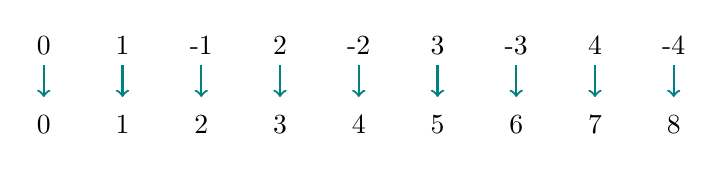
\begin{tikzpicture}

    % Draw the top row of numbers
    \node at (0, 0) {-2};
    \node at (1, 0) {3};
    \node at (-1, 0) {2};
    \node at (2, 0) {-3};
    \node at (-2, 0) {-1};
    \node at (3, 0) {4};
    \node at (-3, 0) {1};
    \node at (4, 0) {-4};
    \node at (-4, 0) {0};

    % Draw the second row of numbers (1, 2, 3, 4, ...)
    \node at (0, -1) {4};
    \node at (1, -1) {5};
    \node at (-1, -1) {3};
    \node at (2, -1) {6};
    \node at (-2, -1) {2};
    \node at (3, -1) {7};
    \node at (-3, -1) {1};
    \node at (4, -1) {8};
    \node at (-4, -1) {0};

    % Draw arrows from the top numbers to the bottom numbers
    \draw[->, teal, thick] (0, -0.25) -- (0, -0.65);
    \draw[->, teal, thick] (1, -0.25) -- (1, -0.65);
    \draw[->, teal, thick] (-1, -0.25) -- (-1, -0.65);
    \draw[->, teal, thick] (2, -0.25) -- (2, -0.65);
    \draw[->, teal, thick] (-2, -0.25) -- (-2, -0.65);
    \draw[->, teal, thick] (3, -0.25) -- (3, -0.65);
    \draw[->, teal, thick] (-3, -0.25) -- (-3, -0.65);
    \draw[->, teal, thick] (4, -0.25) -- (4, -0.65);
    \draw[->, teal, thick] (-4, -0.25) -- (-4, -0.65);

    \end{tikzpicture}
  \end{center}
\end{proof}

\begin{thm}
  $|\mathbb{Q}| = \aleph_0$
\end{thm}

\begin{proof}\leavevmode
  \begin{center}
    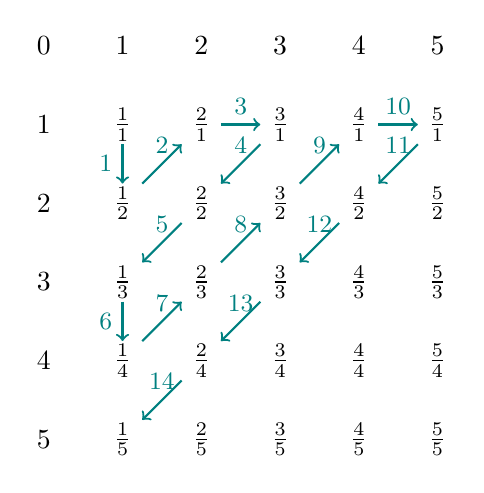
\begin{tikzpicture}

    \def\n{5};

    \foreach \a in {1, ..., \n} {
      \node at (-1, \n-\a) {\a};
    }

    \foreach \a in {1, ..., \n} {
      \node at (\a-1, \n) {\a};
    }

    \node at (-1, \n) {$0$};

    \foreach \a in {1, ..., \n} {
      \foreach \b in {1, ..., \n} {
        \node at (\a-1, -\b+\n) {$\frac{\a}{\b}$};
      }
    }

    \draw[->, teal, thick] (0, \n-1-0.25)       -- node[left]   {\small $1$}    (0, \n-2+0.25);
    \draw[->, teal, thick] (0+0.25, \n-2+0.25)  -- node[above]  {\small $2$}    (1-0.25, \n-1-0.25);
    \draw[->, teal, thick] (1+0.25, \n-1)       -- node[above]  {\small $3$}    (2-0.25, \n-1);
    \draw[->, teal, thick] (2-0.25, \n-1-0.25)  -- node[above]  {\small $4$}    (1+0.25, \n-2+0.25);
    \draw[->, teal, thick] (1-0.25, \n-2-0.25)  -- node[above]  {\small $5$}    (0+0.25, \n-3+0.25);
    \draw[->, teal, thick] (0, \n-3-0.25)       -- node[left]   {\small $6$}    (0, \n-4+0.25);
    \draw[->, teal, thick] (0+0.25, \n-4+0.25)  -- node[above]  {\small $7$}    (1-0.25, \n-3-0.25);
    \draw[->, teal, thick] (1+0.25, \n-3+0.25)  -- node[above]  {\small $8$}    (2-0.25, \n-2-0.25);
    \draw[->, teal, thick] (2+0.25, \n-2+0.25)  -- node[above]  {\small $9$}    (3-0.25, \n-1-0.25);
    \draw[->, teal, thick] (3+0.25, \n-1)       -- node[above]  {\small $10$}   (4-0.25, \n-1);
    \draw[->, teal, thick] (4-0.25, \n-1-0.25)  -- node[above]  {\small $11$}   (3+0.25, \n-2+0.25);
    \draw[->, teal, thick] (3-0.25, \n-2-0.25)  -- node[above]  {\small $12$}   (2+0.25, \n-3+0.25);
    \draw[->, teal, thick] (2-0.25, \n-3-0.25)  -- node[above]  {\small $13$}   (1+0.25, \n-4+0.25);
    \draw[->, teal, thick] (1-0.25, \n-4-0.25)  -- node[above]  {\small $14$}   (0+0.25, \n-5+0.25);

    \end{tikzpicture}
  \end{center}
\end{proof}

\begin{thm}
  $\mathbb{R}$ non è numerabile.
\end{thm}

\begin{proof}[Dimostrazione (Diagonalizzazione di Cantor)]
  Si dimostrerà che $[0, 1]$ non è numerabile. Si supponga di aver trovato un'enumerazione del suddetto insieme. È possibile 
  comunque trovare un nuovo numero nel seguente modo:

  \begin{center}
    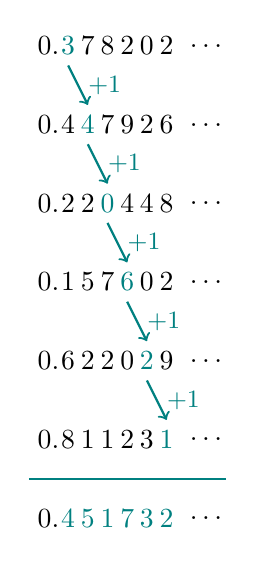
\begin{tikzpicture}

    \node at (-1, 4)  {$0.$};   \node at (-1+0.25, 4)  {$\color{teal} 3$};   \node at (-1+0.5, 4)  {$7$};   \node at (-1+0.75, 4)  {$8$};   \node at (-1+1, 4)  {$2$};   \node at (-1+1.25, 4)  {$0$};    \node at (-1+1.5, 4)  {$2$}; \node at (-1+2, 4)  {$\dots$};
    \node at (-1, 3)  {$0.$};   \node at (-1+0.25, 3)  {$4$};   \node at (-1+0.5, 3)  {$\color{teal} 4$};   \node at (-1+0.75, 3)  {$7$};   \node at (-1+1, 3)  {$9$};   \node at (-1+1.25, 3)  {$2$};    \node at (-1+1.5, 3)  {$6$}; \node at (-1+2, 3)  {$\dots$};
    \node at (-1, 2)  {$0.$};   \node at (-1+0.25, 2)  {$2$};   \node at (-1+0.5, 2)  {$2$};   \node at (-1+0.75, 2)  {$\color{teal} 0$};   \node at (-1+1, 2)  {$4$};   \node at (-1+1.25, 2)  {$4$};    \node at (-1+1.5, 2)  {$8$}; \node at (-1+2, 2)  {$\dots$};
    \node at (-1, 1)  {$0.$};   \node at (-1+0.25, 1)  {$1$};   \node at (-1+0.5, 1)  {$5$};   \node at (-1+0.75, 1)  {$7$};   \node at (-1+1, 1)  {$\color{teal} 6$};   \node at (-1+1.25, 1)  {$0$};    \node at (-1+1.5, 1)  {$2$}; \node at (-1+2, 1)  {$\dots$};
    \node at (-1, 0)  {$0.$};   \node at (-1+0.25, 0)  {$6$};   \node at (-1+0.5, 0)  {$2$};   \node at (-1+0.75, 0)  {$2$};   \node at (-1+1, 0)  {$0$};   \node at (-1+1.25, 0)  {$\color{teal} 2$};    \node at (-1+1.5, 0)  {$9$}; \node at (-1+2, 0)  {$\dots$};
    \node at (-1, -1) {$0.$};   \node at (-1+0.25,-1)  {$8$};   \node at (-1+0.5,-1)  {$1$};   \node at (-1+0.75,-1)  {$1$};   \node at (-1+1,-1)  {$2$};   \node at (-1+1.25,-1)  {$3$};    \node at (-1+1.5,-1)  {$\color{teal} 1$}; \node at (-1+2, -1)  {$\dots$};

    \draw[teal, thick] (-1-0.25, -1.5) -- (-1+2+0.25, -1.5);

    \draw[->, teal, thick] (-1+0.25, 4-0.25)       -- node[right]   {\small $+1$}    (-1+0.5, 3+0.25);
    \draw[->, teal, thick] (-1+0.5, 3-0.25)       -- node[right]   {\small $+1$}    (-1+0.75, 2+0.25);
    \draw[->, teal, thick] (-1+0.75, 2-0.25)       -- node[right]   {\small $+1$}    (-1+1, 1+0.25);
    \draw[->, teal, thick] (-1+1, 1-0.25)       -- node[right]   {\small $+1$}    (-1+1.25, 0+0.25);
    \draw[->, teal, thick] (-1+1.25, 0-0.25)       -- node[right]   {\small $+1$}    (-1+1.5, -1+0.25);

    \node at (-1, -2) {$0.$};   \node at (-1+0.25,-2)  {$\color{teal} 4$};   \node at (-1+0.5,-2)  {$\color{teal} 5$};   \node at (-1+0.75,-2)  {$\color{teal} 1$};   \node at (-1+1,-2)  {$\color{teal} 7$};   \node at (-1+1.25,-2)  {$\color{teal} 3$};    \node at (-1+1.5,-2)  {$\color{teal} 2$}; \node at (-1+2, -2)  {$\dots$};

    \end{tikzpicture}
  \end{center}
\end{proof}

\begin{thm}[Teorema di Cantor]
  Dato un qualsiasi insieme $A$ si ha che $|A| < |\wp{(A)}|$.
\end{thm}

\begin{obs}
  $|\wp{(\mathbb{N})}| = |\mathbb{R}|$. In particolare, $|\mathbb{R}|$ è 
  detta \textbf{cardinalità del continuo}.
\end{obs}

\begin{notation}
  $|\mathbb{R}| = \mathfrak{C}$
\end{notation}

\begin{proof}
  P.A. si supponga che esista $f: A \to \wp{(A)}$ biunivoca. Allora sia $B$ il sottoinsieme 
  di $A$ così definito:

  $$
    B := \{a \in A~\colon~a \not \in f(a)\}
  $$

  dato che $f$ è biunivoca, $\exists b \in A~\colon~f(b) = B$. 
  È facilmente verificabile che $b$ non può né appartenere né non appartenere a $B$, il che è un assurdo.
\end{proof}